\سؤال{نوشتن تست}

برای نوشتن تست در زبان برنامه‌نویسی جاوا، از \lr{junit} استفاده می‌کنیم. برای راه‌اندازی و استفاده از آن در محیط برنامه‌نویسی نرم‌افزار \lr{Intellij} باید به صورت زیر عمل کنیم:
\begin{enumerate}
	\item دو فایل \lr{hamcrest} و \lr{junit} با فرمت \lr{.jar} را دانلود می‌کنیم.
	\item از زبانه‌ی \lr{File} گزینه‌ی \lr{Project Structure} را انتخاب می‌کنیم.
	\begin{figure}[hbpt!]
		\centering
		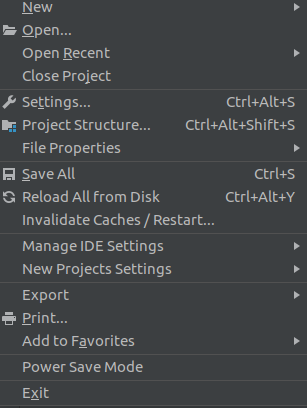
\includegraphics[scale=0.3]{./img/1.png}
	\end{figure}
	\item در قسمت \lr{libraries} در منوی ظاهر شده، دو فایل دانلود شده را اضافه می‌کنیم.
	\begin{figure}[hbpt!]
		\centering
		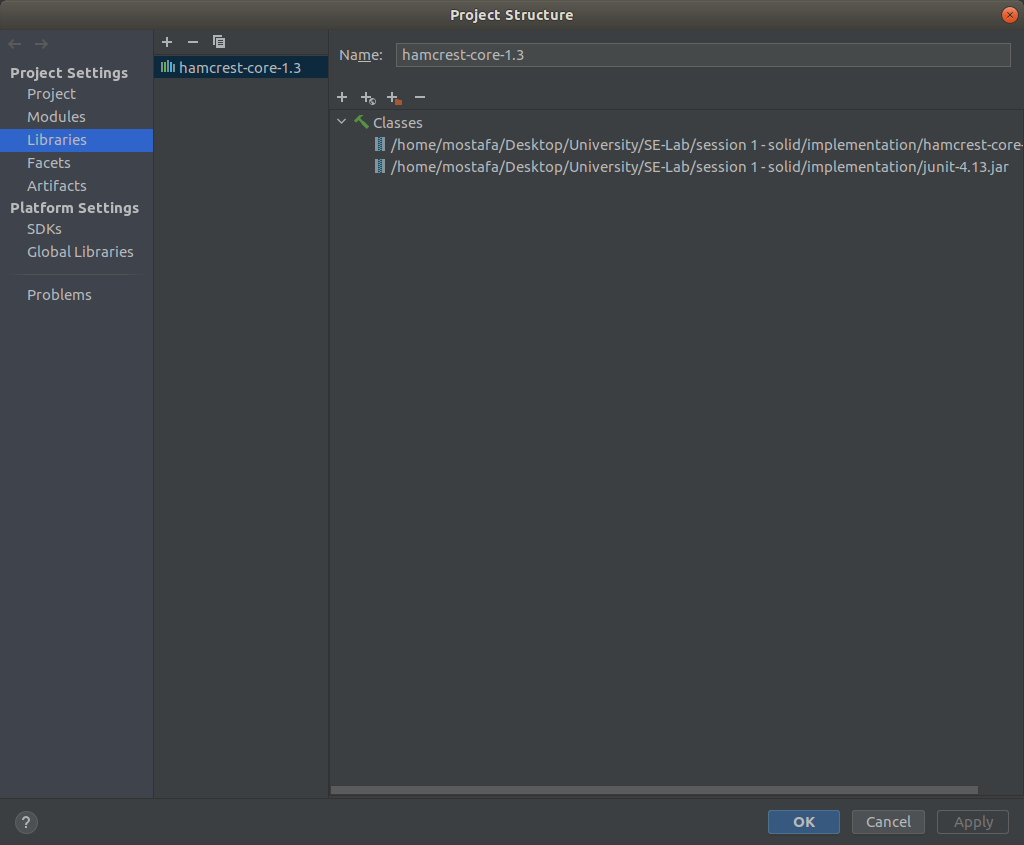
\includegraphics[scale=0.3]{./img/2.png}
	\end{figure}
\end{enumerate}

حال تست‌ها را شروع به نوشتن می‌کنیم. دو عملیات برای اشکال مربع و مستطیل مد نظرمان می‌باشد: 
\begin{itemize}
	\item محاسبه مساحت
	\item تغییر اضلاع
\end{itemize}

برای هر کدام از شکل‌ها باید تستی متناظر با آن را بنویسیم و مقداری که از خروجی آن انتظار می‌رود را امتحان کنیم. لذا مقدار مورد انتظار را با استفاده از متد \lr{assertEquals} از کلاس \lr{Assert} به کار می‌بریم. 

\subsection*{تست محاسبه مساحت مستطیل}
\begin{Verbatim}[tabsize=4]
public class RectangleJUnit {
	@Test
	public void computeArea(){
		Rectangle rectangle = new Rectangle(2, 3);
		double area = rectangle.computeArea();
		Assert.assertEquals(6.0, area, 0.0 );
	}
}
\end{Verbatim}

\subsection*{کد محاسبه مساحت مستطیل}
\begin{Verbatim}[tabsize=4]
public class Rectangle {
	private double width;
	private double height;

	public Rectangle(double width, double height) {
		this.width = width;
		this.height = height;
	}
	
	public double computeArea(){
		return this.width * this.height();
	}
}
\end{Verbatim}

\subsection*{تست تغییر طول مستطیل}
\begin{Verbatim}[tabsize=4]
public class RectangleJUnit {
	@Test
	public void changeWidth() {
		Rectangle rectangle = new Rectangle(3, 4);
		rectangle.setWidth(5);
		Assert.assertEquals(5, rectangle.getWidth(), 0.0 );
	}
}
\end{Verbatim}


\subsection*{تست تغییر عرض مستطیل}
\begin{Verbatim}[tabsize=4]
public class RectangleJUnit {
	@Test
	public void changeHeight() {
		Rectangle rectangle = new Rectangle(3, 4);
		rectangle.setHeight(6);
		Assert.assertEquals(6, rectangle.getHeight(), 0.0 );
	}
}
\end{Verbatim}


\subsection*{تست کلی مستطیل}
\begin{Verbatim}[tabsize=4]
public class RectangleJUnit {
	@Test
	public void computeArea(){
		Rectangle rectangle = new Rectangle(2, 3);
		double area = rectangle.computeArea();
		Assert.assertEquals(6.0, area, 0.0 );
	}
	
	@Test
	public void changeWidth() {
		Rectangle rectangle = new Rectangle(3, 4);
		rectangle.setWidth(5);
		Assert.assertEquals(5, rectangle.getWidth(), 0.0 );
	}
	
	@Test
	public void changeHeight() {
		Rectangle rectangle = new Rectangle(3, 4);
		rectangle.setHeight(6);
		Assert.assertEquals(6, rectangle.getHeight(), 0.0 );
	}
}
\end{Verbatim}

\subsection*{تست محاسبه مساحت مربع}
\begin{Verbatim}
public class SquareJUnit {
	@Test
	public void computeArea(){
		Shape square = new Square(5);
		double area = square.computeArea();
		Assert.assertEquals(25.0, area, 0.0 );
	}
}
\end{Verbatim}
در این قسمت چون کلاس مربع نیز اضافه شده است، برای برقراری اصل \lr{DIP} باید یک \lr{Interface} تعریف کرده و سپس مساحت را به‌گونه‌ی زیر برای کلاس مربع محاسبه کنیم
\subsection*{کد محاسبه مساحت مربع}
\begin{Verbatim}
public class Square implements Shape {
	private double side;
	
	public double computeArea() {
		return this.side * this.side;
	}
}
\end{Verbatim}

\subsection*{تست تغییر ضلع مربع}
\begin{Verbatim}
public class SquareJUnit {
	@Test
	public void changeParameter() {
		Square square = new Square(2);
		square.setSide(4);
		Assert.assertEquals(4.0, square.getSide(), 0.0 );
	}
}
\end{Verbatim}

\subsection*{تست کلی مربع}
\begin{Verbatim}
public class SquareJUnit {
	@Test
	public void computeArea(){
		Shape square = new Square(5);
		double area = square.computeArea();
		Assert.assertEquals(25.0, area, 0.0 );
	}
	
	@Test
	public void changeParameter() {
		Square square = new Square(2);
		square.setSide(4);
		Assert.assertEquals(4.0, square.getSide(), 0.0 );
	}
}
\end{Verbatim}

\subsection*{کد مربوط به رابط شکل}
\begin{Verbatim}
public interface Shape {
	double computeArea();
}
\end{Verbatim}

\subsection*{کد مربوط به مستطیل بعد از تغییر}
\begin{Verbatim}
public class Rectangle implements Shape {
	private double width;
	private double height;
	
	public void setWidth(double width) {
		this.width = width;
	}
	
	public void setHeight(double height) {
		this.height = height;
	}
	
	public double getWidth() {
		return width;
	}
	
	public double getHeight() {
		return height;
	}
	
	public Rectangle(double width, double height) {
		this.setWidth(width);
		this.setHeight(height);
	}
	
	public double computeArea(){
		return this.getWidth() * this.getHeight();
	}

}
\end{Verbatim}


\subsection*{کد مربوط به مربع بعد از تغییر}
\begin{Verbatim}
public class Square implements Shape {
	private double side;
	
	public double getSide() {
		return side;
	}
	
	public void setSide(double side) {
		this.side = side;
	}
	
	public Square(double side){
		this.setSide(side);
	}
	
	public double computeArea() {
		return this.getSide() * this.getSide();
	}

}
\end{Verbatim}


\newpage
\سؤال{اضافه کردن کد اصلی برنامه}

با توجه به این‌که هر دو شکل مربع و مستطیل یک کارایی را برای محاسبه مساحت در نظر دارند؛ بنابراین، یک \lr{Interface} را در نظر گرفتیم که این متد رو به صورت \lr{Abstract} دارد. اگر هر کدام را به عنوان پدر دیگری انتخاب می‌کردیم، از لحاظ اصول‌ اساسی شی‌گرا مشکل پیش می‌آمد و برای برقرار اصل \lr{DIP} این عمل را انجام داده‌ایم.

\subsection*{کد \lr{Shape}}
با توجه به توضیحات داده شده، یک \lr{Interface} با نام \lr{Shape} در نظر گرفته‌ایم که تنها متد آن \lr{computeArea} است.

\begin{Verbatim}[tabsize=4]
public interface Shape {
	double computeArea();
}
\end{Verbatim}



\subsection*{کد \lr{Rectangle}}

\begin{Verbatim}[tabsize=4]
public class Rectangle implements Shape {
	private double width;
	private double height;
	
	public void setWidth(double width) {
		this.width = width;
	}
	
	public void setHeight(double height) {
		this.height = height;
	}
	
	public double getWidth() {
		return width;
	}
	
	public double getHeight() {
		return height;
	}
	
	public Rectangle(double width, double height) {
		this.setWidth(width);
		this.setHeight(height);
	}
	
	public double computeArea(){
		return this.getWidth() * this.getHeight();
	}
}
\end{Verbatim}

\subsection*{کد \lr{Square}}

\begin{Verbatim}[tabsize=4]
public class Square implements Shape {
	private double side;
	
	public double getSide() {
		return side;
	}
	
	public void setSide(double side) {
		this.side = side;
	}
	
	public Square(double side){
		this.setSide(side);
	}
	
	public double computeArea() {
		return this.getSide() * this.getSide();
	}

}
\end{Verbatim}

\newpage
\سؤال{رعایت اصول \lr{SOLID}}

\begin{itemize}
	\item \textbf{\lr{Single Responsibility Principle}}: این اصل برقرار است. زیرا هر کدام از کلاس‌های مستطیل و مربع فقط به یک کنش‌گر جواب‌گو هستند؛ به عبارت دیگر، از هر کدام از متدها فقط یک کنش‌گر استفاده می‌کند. 
	\item \textbf{\lr{Open Closed Principle}}: با توجه به این‌که هر دو کلاس مستطیل و مربع نسبت به تغییرات در منطقشان بسته هستند و در صورتی که بنا به دلایلی در آینده به ارث بخواهند برسند، امکان اضافه کردن قابلیت به آن‌ها وجود دارد.
	\item \textbf{\lr{Liskov Substitution Principle}}: اگر در این قسمت \lr{Interface} را به عنوان کلاس پدر در نظر بگیریم، هر دو کلاس مربع و مستطیل قابلیت جای‌نشینی را دارند. زیرا \lr{precondition}ها قوی‌تر نشده است و هم‌چنین \lr{postcondition}های آن ضعیف‌تر نشده است.
	\item \textbf{\lr{Interface Segregation Principle}}: به دلیل این‌که در این قسمت فقط یک \lr{Interface} داریم، این اصل نیز رعایت می‌شود.
	\item \textbf{\lr{Dependency Inversion Principle}}: همان‌طور که قبلا توضیح داده شد، به دلیل اشتراکاتی که کلاس مربع و کلاس مستطیل دارند، به جای ارث‌بری از یک‌دیگر، از یک واسط برای آن‌ها استفاده کردیم و این اصل رعایت شد.
\end{itemize}